% Chapter Template

\chapter{Introducción} % Main chapter title

\label{Chapter1} % Change X to a consecutive number; for referencing this chapter elsewhere, use \ref{ChapterX}

El ser humano no es consciente del proceso neuronal que tiene lugar en nuestro cerebro con el simple hecho de andar o coger un objeto. Se podría decir que tenemos un super ordenador conectado a los órganos sensoriales capaces de recoger muchísima información y procesarla en un tiempo récord.

Desde la antiguedad ya se estuvo pensando en reproducir las habilidades humanas en algún tipo de máquina, la noción de concebir la mente humana como algún tipo de mecanismo no es reciente es referida en célebres filósofos, sin embargo, no es hasta 1950 y con la noción de la computación cuando se introduce la IA (Inteligencia Artificial) por el científico Alan Turing en su artículo \textit{Maquinaria Computacional e Inteligencia} y donde se empieza a coger interés por este campo que será el precursor de una gran cantidad de desarrollos e innovaciones.

En este proyecto abordaremos el problema de obtener un mapa 3D compacto del
entorno que rodea a nuestro dispositivo a partir de la información aportada por un
sensor RGBD, dando por conocida la información sobre su posición y orientación a
través de algún método externo.

%-----------------------------------
%	SECTION Visión artificial
%-----------------------------------
\section{Visión artificial}

Dentro de la IA, se conoce la visión artificial como el procesado que hace nuestro celebro de las imágenes. Que es actualmente un amplio mundo de investigación y desarrollo. Dispositivos como móviles que usan cámaras (reconocimiento facial).

bajo coste, permite extraer mucha información, procesamiento muy costoso, detección de bordes, features, texturas. Reconocimiento de formas, caras

Aplicaciones:

Medicina
OCR
Biometría
Ojo de halcón (tenis)
MediaPro: distancia recorrida por un futbolista







%-----------------------------------
%	SECTION Técnicas de autolocalización
%-----------------------------------
\section{Técnicas de autolocalización}

Las técnicas de autolocalización ha suscitado gran interés por los investigadores en los últimos años. Consiste en conocer la localización de la cámara en todo momento simplemente con las imágenes capturadas sin disponer de ninguna información extra.

El problema a sido abordado por dos comunidades distintas, por un lado la de visión artificial que denominó al problema como \textbf{structure from motion (SfM)}, donde la información es procesada por lotes, capaz de representar un objeto 2D a 3D con solo unas cuantas imágenes desde diferentes puntos de vista. Y por otro lado la comunidad robótica denominó al problema \textbf{SLAM} (\textit{Simultaneous Localization and Mapping}) que trata de resolver el problema de una manera más compleja adaptando el funcionamiento de los sistemas en tiempo real.

%-----------------------------------
%	SUBSECTION Structure from Motion
%-----------------------------------
\subsection{Structure from Motion (SfM)}

Las técnicas SfM se analizan generalmente de forma offline, las escenas se graban a través de un conjunto de imágenes y luego se procesa, lo que permite realizar optimizaciones para el cálculo de la trayectoria, como por ejemplo el llamado ajuste de haces.

Existen aplicaciones comerciales que utilizan estas técnicas como es el caso de la aplicación PhotoTourism \parencite{Reference2} desarrollada por Microsoft. Que consiste en el cálculo de la posición 3D en la que fueron captadas las imágenes, por ejemplo de un monumento, para después extraer el modelo 3D con el que el usuario puede interactuar libremente (Figura~\ref{fig:Tourism}).

\begin{figure}[th]
\centering
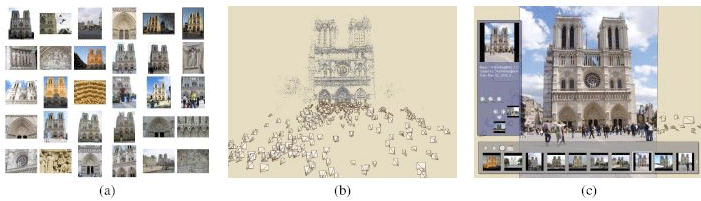
\includegraphics[scale=0.57]{Figures/phototourism.png}
\decoRule
\caption[PhotoTourism]{PhotoTourism: Se recogen una gran colección de imágenes (a), se reconstruyen los puntos 3D y los puntos de vista (b), por último la interfaz permite al usuario interactuar moviendose a través del espacio 3D mediante la transición entre fotografías.}
\label{fig:Tourism}
\end{figure}

%-----------------------------------
%	SUBSECTION Visual SLAM
%-----------------------------------
\subsection{Visual SLAM}

En el problema conocido como \textit{Simultaneous Localization and Mapping} (SLAM) busca resolver los problemas que plantea colocar un robot móvil en un entorno y una posición desconocidas, y que él mismo se encuentre capaz de construir incrementalmente un mapa de su entorno consistente y a la vez utilizar dicho mapa para determinar su propia localización.

La solución a este problema conseguiría hacer sistemas de robots completamente autónomos que junto con un mecanismo de navegación el sistema se encontrará con la capacidad para saber a dónde desplazarse, ser capaz de encontrar obstáculos y reaccionar ante ellos de manera inteligente.

La resolución al problema SLAM ha suscitado un gran interés en el campo de la robótica y ha sido resuelto teóricamente de diversas formas como es el caso del artículo \parencite{Reference1}. Y aunque algunas de ellas han obtenido buenos resultados en la práctica siguen surgiendo problemas a la hora de buscar el método más rápido o el que genere un mejor resultado con menos índice de fallo. La búsqueda de algoritmos y métodos que resuelvan estos problemas sigue siendo una tarea pendiente.

\subsubsection{Odometría visual}

Dentro de las familias de técnicas pertenecientes a las de Visual SLAM se encuentra la de odometría visual, que es la que abordaremos en este trabajo. Consiste en la estimación del movimiento de la cámara en tiempo real. Es decir, el cálculo de la rotación y traslación de la cámara a partir de dos imágenes simultáneas. Se trata de una técnica incremental ya que se basa en la posición anterior para calcular la nueva.

Este tipo de algoritmos se suelen utilizar técnicas de extracción de puntos de interés, cálculos de descriptores y algoritmos para el emparejamiento. Normalmente el proceso es el mismo, una vez calculados los puntos emparejados se calcula la matriz fundamental o esencial y descomponerlas mediante SVD para obtener la matriz de rotación y traslación (RT) (\cite{Reference3}. \cite{Reference4}).

Uno de los trabajos más importantes en el ámbito es el de monoSLAM de Davison\footnote{http://www.doc.ic.ac.uk/\textasciitilde ajd/} \parencite{Reference5} que propone resolver este problema con una única cámara RGB como sensor y realizar el mapeado y la localización simultáneamente. El algoritmo propuesto por Davison utiliza un filtro extendido de Kalman para estimar la posición y la orientación de la cámara, así como la posición de una serie de puntos en el espacio 3D. Para determinar la posición inicial de la cámara es necesario a priori dotar de información con la posición 3D de por lo menos 3 puntos. Después el algoritmo es capaz de situar la cámara en el espacio tridimensional y de generar nuevos puntos para crear el mapa y servir como apoyo a la propia localización de la cámara. En la Figura~\ref{fig:Monoslam} se pueden ver unas capturas de pantalla sobre uno de los experimientos realizados.

\begin{figure}[th]
\centering
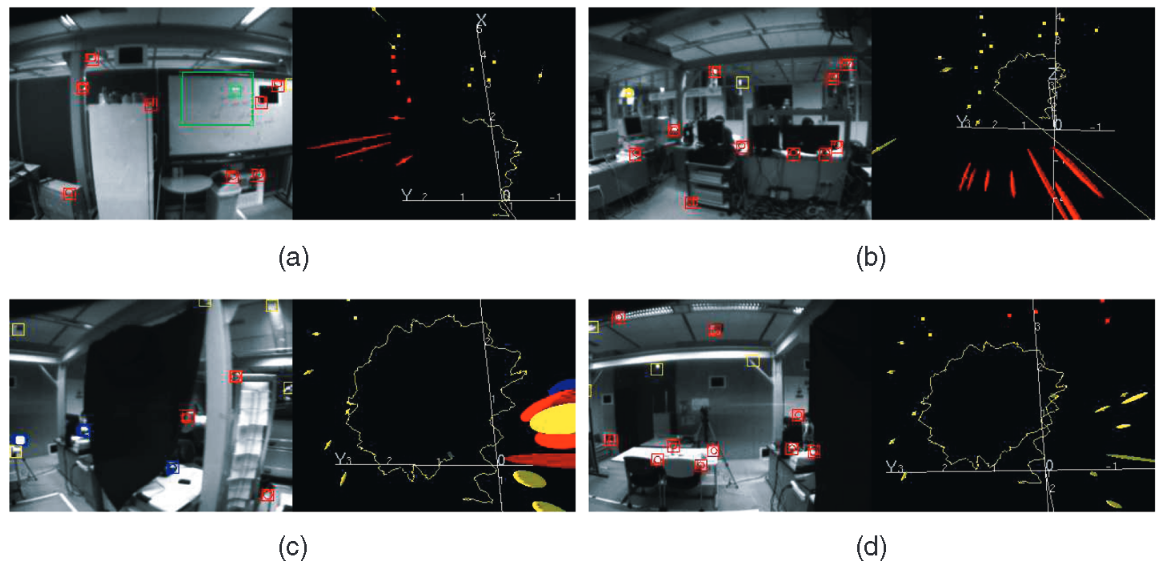
\includegraphics[scale=0.35]{Figures/monoslam.png}
\decoRule
\caption[MonoSlam]{MonoSLAM: Un robot humanoide camina en una trayectoria circular de radio 0.75m. La estela amarilla muestra la trayectoria estimada del robot, y las elipses muestran los errores de localización.}
\label{fig:Monoslam}
\end{figure}

Es importante destacar también la trascendencia que ha tenido el trabajo PTAM \parencite{Reference6} que viene a solucionar uno de los principales problemas que tienen los algoritmos monoSLAM; el tiempo de cómputo, ya que aumenta exponencialmente con el número de puntos (Figura~\ref{fig:Ptam}). Para ello se aborda el problema separando el mapeado de la localización, de tal modo que solo la localización deba funcionar en tiempo real, dejando así que el mapeado trabaje de una manera asíncrona. Este algoritmo parte de la idea de que solo la localización es necesaria que funcione en tiempo real. PTAM hace uso de \textit{keyframes}, es decir, fotogramas clave que se utilizan tanto para la localización como para el mapeado y también de una técnica de optimización mediante ajuste de haces, como en SfM.

\begin{figure}[th]
\centering
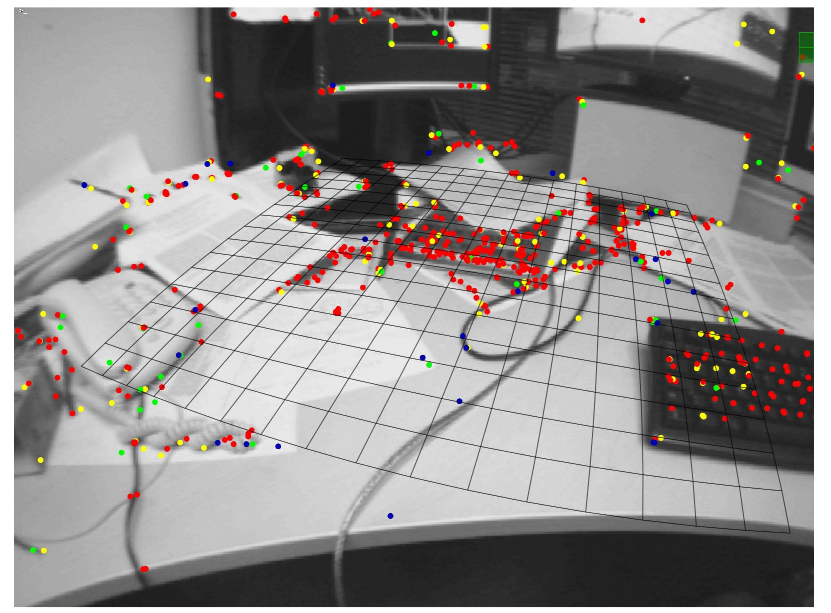
\includegraphics[scale=0.4]{Figures/ptam.png}
\decoRule
\caption[Ptam]{PTAM: Funcionamiento típico del sistema sobre un escritorio.}
\label{fig:Ptam}
\end{figure}

%-----------------------------------
%	SECTION Realidad aumentada
%-----------------------------------
\section{Realidad aumentada}